\documentclass[11pt,letterpaper,boxed]{hmcpset}
\usepackage{fullpage}
\setlength{\parskip}{6pt}
\setlength{\parindent}{0pt}
\usepackage[margin=1in]{geometry}
\usepackage{graphicx}
\usepackage{enumerate}
\usepackage{marvosym}
\usepackage{amssymb}
\usepackage{wasysym}
\usepackage{gensymb}
\usepackage{mathrsfs}
\usepackage{scrextend}
\usepackage{mathtools}
\usepackage{pgfplots}
\usepackage{xspace}
\usepackage{esvect}
\usepackage{lipsum}
\usepackage{float}
\usepackage{esint}
\usepackage{inputenc}

\name{Name $\rule{4cm}{0.15mm}$}
\class{Physics 51M Section $\rule{.5cm}{0.15mm}$ Box \# $\rule{1cm}{0.15mm}$}
\assignment{Problem Set 6}
\duedate{28 October 2019}

\begin{document}
	
	%\begin{center}
	\noindent\textbf{Collaborators:} 
	%\end{center} 
	
	%\problemlist{}
	
	\begin{problem} [Problem 1]
		During a thunderstorm, clouds become negatively charged on the bottom (via some as yet poorly understood process) and induces a corresponding positive charge on the surface of the Earth directly below the cloud, as shown in the figure. A typical thundercloud has a charge of $-20$ C in the bottom layer and a bottom surface area around $50$ km$^2$. Assume that the bottom of the cloud is roughly 
		$1$ km above the Earth’s surface.
		\begin{enumerate}
			\item [(a)] Treating the charged layers as a parallel plate capacitor, find the electric field in the air underneath the thundercloud.
			\item [(b)] How much energy is stored in one cubic meter of air, in the region underneath the thundercloud. Comment on your result. 
			\item [(c)]  When the electric field is high enough, it can ionize the air between the Earth’s surface and the cloud. The resulting discharge is the phenomenon we know as lightning. If all the excess negative charge is transferred from the cloud to the ground, estimate the net energy released in this event.
		\end{enumerate}

		\begin{center}
		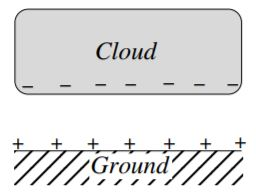
\includegraphics[scale=.7]{51m6pic.jpg}
		\end{center}
		
	\end{problem}
	
	\begin{solution}
		\vfill
	\end{solution}
	\newpage
	
	\begin{problem} [Problem 2]
		The electrostatic potential V in the space between the plates of a particular, and now obsolete,
		vacuum tube is given by V = (1530 V/$m^2$)$x^2$, where $x$ is the distance from one of the plates.
		\begin{enumerate}
			\item [(a)] Calculate the magnitude and direction of the electric field at $x = 1.5 cm$.
			\item [(b)] Determine the volume charge density $\rho$ between the plates, and the surface charge density on each of the plates, assuming one plate is at $x = 0$ and the other is at $x = 1.5 cm$. Consider the plates to be metal conductors of finite thickness.
		\end{enumerate}

	\end{problem}
	
	\begin{solution}
	\vfill
	\end{solution}
	\newpage

	\begin{problem}[Problem 3*]
		Consider a solid non-conducting sphere of radius R, corrying a uniform negative charge density and total charge $-q$.
		\begin{enumerate}
			\item [(a)] Find the electric field inside and outside the sphere.
			\item [(b)] Find the electrostatic potential everywhere in space, taking $V = 0$ at infinity.
		\end{enumerate}
	
	\end{problem}
	
	\begin{solution}
	\vfill
	\end{solution}
	\newpage

	\begin{problem} [Problem 4]
		Consider a spherical conductor of radius a centered inside a spherical conducting shell of inner radius $b$ and outer radius $c$, as shown in the figure. The outer conductor is grounded, that is, its potential is held fixed at $V = 0$; the potential at infinity is also taken to be 0. The inner conductor has a potential $+V_0$.
		\begin{enumerate}
			\item [(a)] Find the potential everywhere in space and sketch $V(r)$ vs. $r$.
			\item [(b)] Find the charge on the inner conductor in term of the given quantities.
			\item [(c)] Find the net charge on the outer conducting shell and describe the charge distribution. (Hint: The Earth ground acts as an infinite reservoir of charge.)
			\item [(d)] How much kinetic energy would a charge $+Q$ gain/lose if it traveled from the inner sphere to the outer shell?
		\end{enumerate}
	
		\begin{center}
		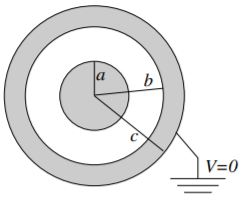
\includegraphics[scale=.7]{51m6pic2.jpg}
		\end{center}
	
	\end{problem}
	
	\begin{solution}
	\vfill
	\end{solution}
	\newpage

	\begin{problem} [Problem 5]
		\begin{enumerate}
			\item [(a)] Calculate the energy density of the electric field at a distance $r$ from an electron (presumed
			to be a point particle) at rest.
			\item [(b)] Assume now that the electron is not a point but a sphere of radius $R$ over whose surface the electron charge is uniformly distributed. Determine the energy associated with the external electric field in vacuum of the electron as a function of R.
			\item [(c)] If you now associate this energy with the mass of the electron, you can, using $E_0 = mc^2$, calculate a value for $R$. Evaluate this radius numerically; it is often called the classical radius of the electron.
		\end{enumerate}
	
	\end{problem}
	
	\begin{solution}
	\vfill
	\end{solution}
	\newpage

	\begin{problem} [Problem 6]
		A dielectric material with dielectric constant $K_e$ is placed in the interior of a parallel plate capacitor. Assume there is a free surface charge $\pm \sigma$ on the plates of the capacitor. What is the polarization charge induced on each surface of the dielectric, $\sigma_pol$? Determine your answer using Gauss's law and the definition of the dielectric constant: $K_e = \frac{E_0}{E_{dielectric}}$.
	\end{problem}
	
	\begin{solution}
	\vfill
	\end{solution}
	\newpage




\end{document}
